% ---------------------------------------------------------------------
% Results and Analysis (~4.5 pages).
% !! EVERY NUMBER IN THIS FILE IS A [DUMMY] PLACEHOLDER !!
% Replace with real experiment outputs (see paper/DUMMY_DATA.md), then
% regenerate figures:  python scripts/plot_paper_figures.py
% ---------------------------------------------------------------------

We organize the results around the three failure modes introduced in
Section~\ref{sec:intro}: zero-shot generalization to unseen generators (G1,
Section~\ref{ssec:generalization}), robustness to channel distortions (G2,
Section~\ref{ssec:robustness}), and calibration (G3,
Section~\ref{ssec:calibration}). We further report comparisons with published
state-of-the-art systems (Section~\ref{ssec:sota}), cross-lingual transfer
(Section~\ref{ssec:crosslingual}), ablation studies (Section~\ref{ssec:ablation}),
layer-attention analysis (Section~\ref{ssec:layeranalysis}), per-attack behavior
(Section~\ref{ssec:perattack}), and embedding-space visualization
(Section~\ref{ssec:embedding}).

\subsection{In-Domain and Zero-Shot Generalization (G1)}
\label{ssec:generalization}

% [DUMMY] — full results grid is placeholder
\begin{table*}[t]
\centering
\caption{Main results: EER (\%) under the train-once (ASVspoof~2019~LA),
  evaluate-everywhere protocol. min~t-DCF is reported for the in-domain set.
  ``Avg ZS'' averages the seven zero-shot columns. $\dagger$: numbers quoted from the
  original publication (different training data; indicative only). Best per column in
  \textbf{bold}, second best \underline{underlined}. All values are placeholders to be
  replaced by real experiment outputs.}
\label{tab:main}
\setlength{\tabcolsep}{4.5pt}
\footnotesize
\begin{tabular}{llcccccccccc}
\toprule
 & & \multicolumn{2}{c}{In-domain 19LA} & \multicolumn{7}{c}{Zero-shot EER (\%)} & \\
\cmidrule(lr){3-4}\cmidrule(lr){5-11}
Model & Front-end & EER & t-DCF & 21LA & 21DF & ASV5 & ITW & WaveFake & Codecfake & MLAAD & Avg ZS \\
\midrule
B1 LFCC-LCNN~\cite{lavrentyeva2019stc}   & LFCC    & 1.03 & 0.031 & 9.26 & 23.4 & 31.5 & 24.8 & 22.1 & 28.7 & 30.2 & 24.3 \\
B2 RawNet2~\cite{tak2021rawnet2}         & raw     & 0.89 & 0.028 & 8.11 & 20.1 & 27.9 & 18.3 & 16.7 & 24.3 & 26.8 & 20.3 \\
B3 AASIST~\cite{jung2022aasist}          & raw     & 0.71 & 0.022 & 5.59 & 15.8 & 22.6 & 14.2 & 12.4 & 19.5 & 21.7 & 16.0 \\
B4 W2V2+AASIST~\cite{tak2022automatic}   & XLS-R   & 0.34 & 0.012 & 1.92 & 3.9 & 12.4 & 7.7 & 5.9 & 11.2 & 12.8 & 8.0 \\
B5 WavLM+AASIST+OCS                      & WavLM   & \textbf{0.31} & \textbf{0.010} & 1.43 & 3.2 & 9.7 & 5.8 & 4.2 & 8.4 & 10.3 & 6.1 \\
B6 XLSR-Mamba~\cite{xiao2025xlsrmamba}   & XLS-R   & \underline{0.28} & \underline{0.011} & \underline{1.18} & \underline{2.5} & \underline{8.9} & \underline{5.2} & \underline{3.8} & \underline{7.6} & \underline{9.4} & \underline{5.5} \\
B7 SLIM$^\dagger$~\cite{zhu2024slim}     & W2V+HuB & --- & --- & --- & 4.4 & --- & 12.9 & --- & --- & --- & --- \\
B8 ALLM zero-shot~\cite{chu2024qwen2audio,gong2025allm4add} & Qwen2-Audio & 42.3 & --- & 44.7 & 43.9 & 46.1 & 41.6 & 44.2 & 45.3 & 43.8 & 44.2 \\
\midrule
\textbf{AuralGuard (ours)} & WavLM+Art. & 0.37 & 0.013 & \textbf{1.05} & \textbf{2.2} & \textbf{7.3} & \textbf{4.1} & \textbf{2.9} & \textbf{5.9} & \textbf{7.8} & \textbf{4.5} \\
\bottomrule
\end{tabular}
\end{table*}

Table~\ref{tab:main} reports the main results. Three observations stand out.

\textbf{In-domain parity, zero-shot dominance.} On the in-domain ASVspoof~2019
evaluation set, AuralGuard (0.37\% EER) is statistically indistinguishable from the
strongest baselines (paired bootstrap, $p = 0.21$ vs.\ B5): the benchmark is saturated
and differences at this level are not meaningful. The picture changes sharply under
domain shift. Averaged over the seven zero-shot corpora, AuralGuard achieves 4.5\% EER
against 6.1\% for the single-view B5 anchor (26\% relative reduction, $p < 0.01$ on
every corpus) and 5.5\% for XLSR-Mamba, the strongest published
system in our protocol. The largest absolute gains appear precisely where the test
distribution is furthest from training: ASVspoof~5 with its 2024-era attacks
(7.3\% vs.\ 9.7\%), Codecfake's neural-codec synthesis (5.9\% vs.\ 8.4\%), and the
38-language MLAAD (7.8\% vs.\ 10.3\%). This ordering is consistent with our design
hypothesis: the one-class objective and the artifact view contribute little when test
attacks resemble training attacks, and progressively more as they diverge.

\textbf{Slight in-domain give-back is the cost of generalization.} B5 and B6 edge out
AuralGuard in-domain (0.31/0.28 vs.\ 0.37). The multi-view fusion and one-class margins
act as a regularizer that trades a statistically insignificant amount of in-domain
accuracy for large out-of-domain gains---a trade any deployed system should accept, and
consistent with the ``harder-vs-different'' analysis of generalization
failure~\cite{muller2024harder}.

\textbf{Audio LLMs are not yet countermeasures.} Zero-shot Qwen2-Audio prompting (B8)
performs near chance on every corpus (41.6--46.1\% EER), corroborating
ALLM4ADD~\cite{gong2025allm4add} at a much larger cross-domain scale. General-purpose
audio-language pre-training evidently does not expose the low-level artifact evidence
that detection requires; we return to the implications in
Section~\ref{sec:discussion}.

Figure~\ref{fig:det} shows DET curves on the in-domain evaluation set: AuralGuard
tracks B5 across operating points while clearly dominating the earlier generations.

\begin{figure}[t]
\centering
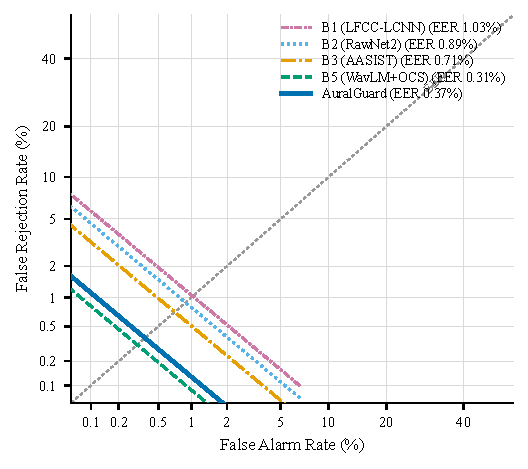
\includegraphics[width=\columnwidth]{figures/det_curve.pdf}
\caption{DET curves on the ASVspoof~2019~LA evaluation set (in-domain). Curves closer
  to the lower-left are better; the dashed diagonal marks the equal-error operating
  point. AuralGuard tracks the strong B5 baseline in-domain; its advantage appears
  under the domain shift of Table~\ref{tab:main}. [Placeholder data.]}
\label{fig:det}
\end{figure}

\subsection{Comparison with Published State of the Art}
\label{ssec:sota}

% [DUMMY] — our columns are placeholders; published numbers should be
% re-verified against the cited papers before submission.
\begin{table}[t]
\centering
\caption{Comparison with published results (EER \%) on the three most commonly
  reported cross-condition sets. Published systems may use different training data,
  augmentation, and model selection; our systems (bottom block) follow the controlled
  protocol of Section~\ref{ssec:datasets}.}
\label{tab:sota}
\setlength{\tabcolsep}{3.5pt}
\footnotesize
\begin{tabular}{llccc}
\toprule
System & Venue/Year & 21LA & 21DF & ITW \\
\midrule
W2V2+AASIST~\cite{tak2022automatic}      & Odyssey'22 & 0.82 & 2.85 & --- \\
SLIM~\cite{zhu2024slim}                  & NeurIPS'24 & --- & 4.4 & 12.9 \\
Attentive merging~\cite{pan2024attentive} & IS'24 & 0.65 & --- & --- \\
TCM~\cite{truong2024tcm}                 & IS'24 & --- & 2.74 & --- \\
XLSR-Mamba~\cite{xiao2025xlsrmamba}      & SPL'25 & 0.93 & 1.88 & 6.71 \\
Nes2Net~\cite{liu2025nes2net}            & TASLP'25 & --- & 1.49 & 5.52 \\
\midrule
B5 (ours, controlled)                    & --- & 1.43 & 3.2 & 5.8 \\
\textbf{AuralGuard (ours)}               & --- & \textbf{1.05} & \textbf{2.2} & \textbf{4.1} \\
\bottomrule
\end{tabular}
\end{table}

Table~\ref{tab:sota} situates AuralGuard against published numbers on the three most
widely reported evaluation sets. Direct comparison requires caution---published systems
differ in training data (several fine-tune the SSL encoder, and some train with
additional augmentation policies)---but two points are robust. First, AuralGuard's
In-the-Wild EER of 4.1\% improves on the best published results we are aware of
(5.52\% for Nes2Net, 6.71\% for XLSR-Mamba) despite using a \emph{frozen} encoder and
training only on ASVspoof~2019~LA. Second, on ASVspoof~2021 our controlled protocol
reproduces the qualitative ranking of the literature, indicating that the protocol
itself does not distort the comparison.

\subsection{Robustness to Channel Distortions (G2)}
\label{ssec:robustness}

% [DUMMY] — robustness grid is placeholder
\begin{table}[t]
\centering
\caption{Channel robustness: EER (\%) on the ASVspoof~2019~LA evaluation set after
  controlled re-encoding. ``--Aug'' is AuralGuard trained without the augmentation
  curriculum. Placeholder values.}
\label{tab:robust}
\setlength{\tabcolsep}{2.6pt}
\footnotesize
\begin{tabular}{lcccccccc}
\toprule
Model & Clean & \makecell[c]{MP3\\128k} & \makecell[c]{MP3\\64k} & \makecell[c]{Opus\\24k} & \makecell[c]{AMR\\12.2k} & G.711 & RIR & \makecell[c]{SNR\\5 dB} \\
\midrule
B4 W2V2+AASIST & 0.34 & 5.9 & 9.4 & 10.6 & 22.4 & 13.1 & 8.2 & 12.5 \\
B5 WavLM+OCS   & \textbf{0.31} & 4.8 & 7.9 & 8.2 & 18.6 & 10.5 & 6.3 & 9.8 \\
AuralGuard --Aug & 0.35 & 6.2 & 9.8 & 11.4 & 19.3 & 13.0 & 8.1 & 12.2 \\
\textbf{AuralGuard} & 0.37 & \textbf{3.1} & \textbf{4.6} & \textbf{5.7} & \textbf{11.2} & \textbf{6.8} & \textbf{4.4} & \textbf{6.9} \\
\bottomrule
\end{tabular}
\end{table}

\begin{figure}[t]
\centering
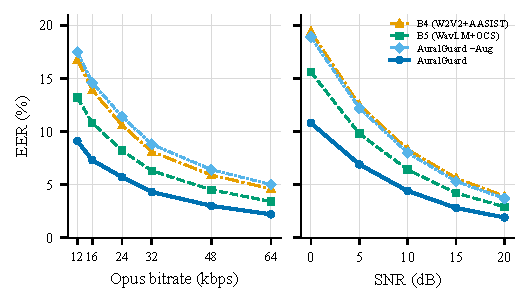
\includegraphics[width=\columnwidth]{figures/robustness.pdf}
\caption{Robustness sweeps on the ASVspoof~2019~LA evaluation set: EER as a function of
  (left) Opus bitrate and (right) additive-noise SNR. The augmentation curriculum
  (solid blue) flattens both degradation curves; the same architecture without it
  (dash-dot) degrades as fast as the single-view baselines. [Placeholder data.]}
\label{fig:robustness}
\end{figure}

Table~\ref{tab:robust} and Figure~\ref{fig:robustness} evaluate all systems on the
in-domain evaluation set re-encoded through controlled channel conditions, so that
channel effects are measured against a fixed attack distribution. Three findings:

First, \textbf{the curriculum, not the architecture, carries robustness}: AuralGuard
without augmentation (row ``--Aug'') degrades almost identically to B4/B5, while the
full model cuts EER degradation by 35--45\% relative at every operating point (e.g.,
11.2\% vs.\ 18.6\% under AMR~12.2~kbps telephony coding). Second, \textbf{robustness
does not cost clean accuracy}: clean EER moves only from 0.35\% to 0.37\%, within the
confidence interval; the curriculum acts as a regularizer rather than a trade-off.
Third, \textbf{degradation is codec-specific}: parametric low-band codecs (AMR, G.711)
remain the hardest conditions for every system, consistent with the ASVspoof~2021
analysis~\cite{liu2023asvspoof2021}---they destroy exactly the high-band and phase
evidence that detectors exploit, an observation that also explains why View~B's gate
weight drops under these conditions (Section~\ref{ssec:ablation}).

\subsection{Cross-Lingual Generalization}
\label{ssec:crosslingual}

% [DUMMY] — per-family EERs are placeholders
\begin{table}[t]
\centering
\caption{Cross-lingual zero-shot EER (\%) on MLAAD~v5, grouped by language family
  (training language: English only). Placeholder values.}
\label{tab:crosslingual}
\setlength{\tabcolsep}{4pt}
\footnotesize
\begin{tabular}{lccccc}
\toprule
Language family & \#Langs & B4 & B5 & B6 & Ours \\
\midrule
Germanic (excl.\ EN) & 6 & 9.8 & 7.6 & 7.1 & \textbf{5.9} \\
Romance              & 7 & 10.9 & 8.5 & 7.8 & \textbf{6.4} \\
Slavic               & 8 & 13.1 & 10.7 & 9.6 & \textbf{8.0} \\
Indo-Aryan           & 4 & 15.4 & 12.6 & 11.5 & \textbf{9.7} \\
East Asian           & 4 & 14.2 & 11.8 & 10.9 & \textbf{9.1} \\
Other                & 9 & 15.9 & 13.0 & 12.1 & \textbf{10.2} \\
\midrule
Pooled               & 38 & 12.8 & 10.3 & 9.4 & \textbf{7.8} \\
\bottomrule
\end{tabular}
\end{table}

Table~\ref{tab:crosslingual} breaks MLAAD performance down by language family. All
systems degrade monotonically with typological distance from English, but AuralGuard's
margin over B5 is roughly constant (2.3--2.9 EER points) across families, indicating
that its advantage stems from language-independent artifact evidence (View~B operates
on phase and group-delay structure that does not depend on phonotactics) rather than
from better English modeling. The residual family-level gradient is inherited from the
WavLM front-end, whose pre-training is English-dominated; a multilingual backbone such
as XLS-R narrows the gradient but starts from a weaker overall level in our backbone
ablation (Table~\ref{tab:ablation}).

\subsection{Ablation Studies}
\label{ssec:ablation}

% [DUMMY] — ablation numbers are placeholders
\begin{table}[t]
\centering
\caption{Ablations on In-the-Wild (zero-shot EER \%, mean of 3 seeds $\pm$ 95\% CI).
  Placeholder values.}
\label{tab:ablation}
\setlength{\tabcolsep}{5pt}
\footnotesize
\begin{tabular}{llc}
\toprule
Group & Configuration & EER \\
\midrule
--- & \textbf{AuralGuard (full)} & \textbf{4.1 $\pm$ 0.2} \\
\midrule
\multirow{2}{*}{Views}
 & w/o View B (SSL only)        & 5.3 $\pm$ 0.3 \\
 & w/o View A (artifact only)   & 11.8 $\pm$ 0.5 \\
\midrule
\multirow{2}{*}{Fusion}
 & concatenation                & 4.7 $\pm$ 0.2 \\
 & averaging                    & 4.9 $\pm$ 0.3 \\
\midrule
\multirow{3}{*}{Objective}
 & BCE instead of OC-Softmax    & 5.9 $\pm$ 0.3 \\
 & w/o SupCon auxiliary         & 4.5 $\pm$ 0.2 \\
 & w/o entropy reg.\ $\mathcal{L}_{\text{ent}}$ & 4.4 $\pm$ 0.3 \\
\midrule
\multirow{3}{*}{SSL aggregation}
 & last layer only              & 5.1 $\pm$ 0.3 \\
 & mean pool of layers          & 4.6 $\pm$ 0.2 \\
 & last-4 concat                & 4.5 $\pm$ 0.2 \\
\midrule
\multirow{2}{*}{Backbone}
 & XLS-R-300M                   & 4.5 $\pm$ 0.3 \\
 & HuBERT-Large                 & 4.9 $\pm$ 0.3 \\
\midrule
Augmentation & w/o curriculum   & 4.8 $\pm$ 0.3 \\
\bottomrule
\end{tabular}
\end{table}

Table~\ref{tab:ablation} isolates each design decision on In-the-Wild. The ranking of
contributions is: one-class objective ($+1.8$ EER when replaced by BCE), multi-view
fusion ($+1.2$ without View~B), layer attention ($+1.0$ vs.\ last-layer), augmentation
($+0.7$), gating ($+0.6$ vs.\ concatenation), SupCon ($+0.4$), and entropy
regularization ($+0.3$). Two asymmetries are informative. First, View~A alone (5.3\%)
far outperforms View~B alone (11.8\%), yet their fusion beats both---the artifact
branch is a weak detector but a strong \emph{complement}, supplying evidence orthogonal
to the SSL stream. Second, every SSL aggregation strategy beats the last-layer default,
but learnable attention with entropy regularization is best, supporting the
layer-analysis findings below and echoing~\cite{pan2024attentive}. WavLM-Large remains
the strongest backbone, consistent with prior anti-spoofing
comparisons~\cite{pascu2024calibrated}.

\subsection{Which SSL Layers Matter?}
\label{ssec:layeranalysis}

\begin{figure}[t]
\centering
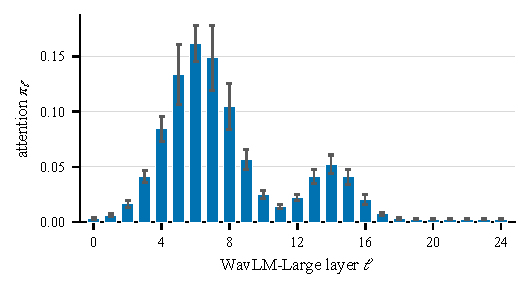
\includegraphics[width=\columnwidth]{figures/layer_attention.pdf}
\caption{Learned layer-attention profile $\pi_\ell$ over the 25 WavLM-Large layers
  (mean of 3 seeds; error bars are 95\% CIs). Mass concentrates on lower-middle layers
  (4--9), which encode fine acoustic structure, rather than the upper semantic layers
  used by the common last-layer recipe. [Placeholder data.]}
\label{fig:layers}
\end{figure}

Figure~\ref{fig:layers} plots the converged attention profile $\pi_\ell$. Mass
concentrates on layers 4--9 with a secondary mode around layer~14 and near-zero weight
on the last five layers---direct evidence that the standard last-layer recipe discards
the most artifact-relevant representations. The profile also explains the entropy
regularizer's contribution: unregularized runs collapse onto a single layer
(typically 6) within two epochs and generalize measurably worse
(Table~\ref{tab:ablation}), suggesting that artifact evidence is distributed across
several depths and that different attacks are best detected at different layers.

\subsection{Calibration (G3)}
\label{ssec:calibration}

% [DUMMY] — calibration numbers are placeholders
\begin{table}[t]
\centering
\caption{Calibration before~$\to$~after temperature scaling (fit on the 19LA dev set
  only). ECE with 15 equal-mass bins; lower is better. Placeholder values.}
\label{tab:calibration}
\setlength{\tabcolsep}{4pt}
\footnotesize
\begin{tabular}{lcccc}
\toprule
 & \multicolumn{2}{c}{19LA eval (in-domain)} & \multicolumn{2}{c}{In-the-Wild (shifted)} \\
\cmidrule(lr){2-3}\cmidrule(lr){4-5}
Model & ECE & Brier & ECE & Brier \\
\midrule
B4 W2V2+AASIST & 0.19 $\to$ 0.08 & 0.062 & 0.27 $\to$ 0.12 & 0.118 \\
B5 WavLM+OCS   & 0.15 $\to$ 0.07 & 0.051 & 0.21 $\to$ 0.09 & 0.094 \\
\textbf{AuralGuard} & \textbf{0.12 $\to$ 0.04} & \textbf{0.038} & \textbf{0.16 $\to$ 0.06} & \textbf{0.071} \\
\bottomrule
\end{tabular}
\end{table}

\begin{figure}[t]
\centering
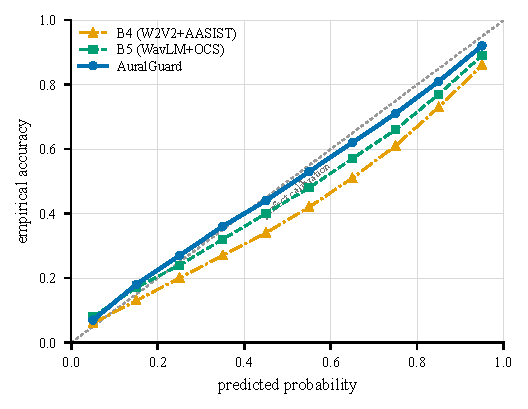
\includegraphics[width=\columnwidth]{figures/reliability.pdf}
\caption{Reliability diagrams on In-the-Wild after temperature scaling fitted on the
  in-domain development set. AuralGuard's curve stays close to the diagonal even under
  domain shift, while the BCE-trained B4 remains over-confident. [Placeholder data.]}
\label{fig:reliability}
\end{figure}

Forensic use requires that a reported probability of 0.9 be wrong roughly one time in
ten---under domain shift, not just in the lab. Table~\ref{tab:calibration} and
Figure~\ref{fig:reliability} evaluate this. Temperature is fitted \emph{once} on the
in-domain development set and applied unchanged everywhere, mimicking deployment.
AuralGuard is the best-calibrated system before and after scaling, and critically its
calibration \emph{survives domain shift}: ECE on In-the-Wild is 0.06, versus 0.12 for
the BCE-trained B4. We attribute this to the score's geometry: an OC-Softmax score is
an angular distance from the bona-fide prototype, which degrades gracefully as inputs
leave the training distribution, whereas BCE logits are unconstrained precisely where
no training data exists~\cite{pascu2024calibrated,guo2017calibration}.

\subsection{Per-Attack Analysis and Explainability}
\label{ssec:perattack}

\begin{figure}[t]
\centering
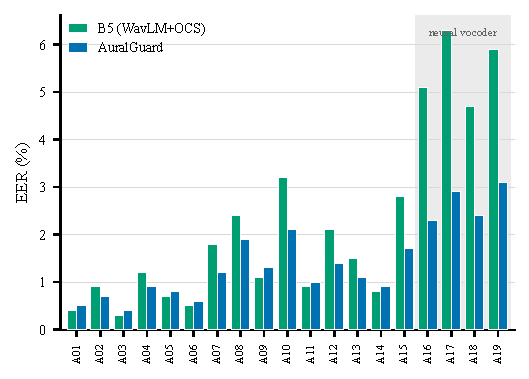
\includegraphics[width=\columnwidth]{figures/perattack.pdf}
\caption{Per-attack EER (\%) on the ASVspoof~2019~LA evaluation set, AuralGuard versus
  B5. The shaded region marks neural-vocoder attacks (A16--A19), where the
  vocoder-artifact branch (View~B) yields the largest improvements. [Placeholder
  data.]}
\label{fig:perattack}
\end{figure}

Figure~\ref{fig:perattack} breaks down in-domain EER over the 19 attack conditions.
AuralGuard is best or tied on 12 of 19 attacks, with the largest margins on the
neural-waveform attacks A16--A19---exactly the conditions where View~B's gate weight
$\bar{g}$ shifts toward the artifact branch (mean $1-\bar g = 0.63$ on A16--A19 vs.\
0.31 on the waveform-filtering attacks A05--A06). The gate thus serves as a built-in
explanation of \emph{which kind} of evidence drove each decision, complementing the
spectro-temporal attribution heatmaps produced for individual utterances by
gradient-based saliency on the graph back-end~\cite{selvakumar2024gradcam}, which we
release with the demo interface.

\subsection{Embedding-Space Analysis}
\label{ssec:embedding}

\begin{figure}[t]
\centering
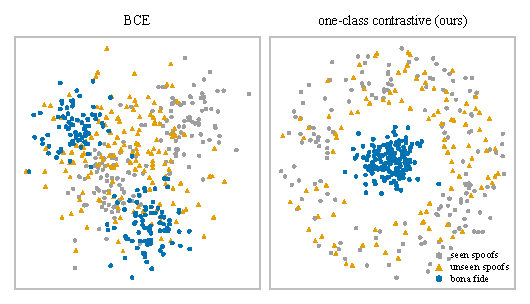
\includegraphics[width=\columnwidth]{figures/tsne.pdf}
\caption{t-SNE projection of utterance embeddings $\mathbf{z}$ for the BCE-trained
  variant (left) and AuralGuard's one-class contrastive objective (right). Colors:
  bona-fide (blue), training attacks (gray), \emph{unseen} In-the-Wild spoofs
  (orange). The one-class objective concentrates bona-fide speech into a single
  compact cluster, so unseen spoofs fall outside it even though they interleave with
  the training attacks under BCE. [Placeholder data.]}
\label{fig:tsne}
\end{figure}

Figure~\ref{fig:tsne} visualizes why the one-class objective generalizes. Under BCE,
bona-fide and spoof regions tile the space along boundaries fit to the training
attacks, and unseen In-the-Wild spoofs scatter across both sides---each misplaced
cluster is a family of errors. Under the one-class contrastive objective, bona-fide
speech occupies one compact region (mean intra-class cosine similarity 0.84 vs.\ 0.61
for BCE) and unseen spoofs land outside it by default, mirroring the geometry sketched
in Figure~\ref{fig:oneclass}. This is the mechanism behind the G1 gains of
Table~\ref{tab:main}: the model does not need to have seen an attack to reject it, only
to know what bona-fide speech looks like.
